\begin{figure}[h]
		\begin{center}
			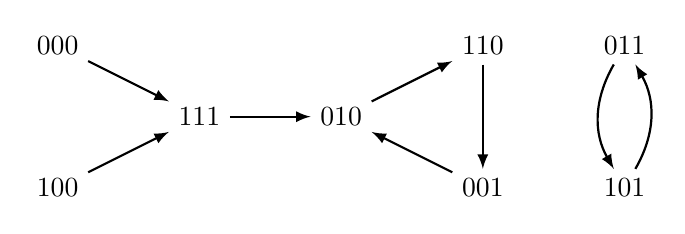
\begin{tikzpicture}[scale=.9]
				\draw (0,2) node (1) {000};
				\draw (2,1) node (2) {111};
				\draw (4,1) node (3) {010};
				\draw (8,2) node (4) {011};
				\draw (0,0) node (8) {100};
				\draw (6,0) node (7) {001};
				\draw (6,2) node (6) {110};
				\draw (8,0) node (5) {101};
				\draw[-latex, thick] (1) -- (2);
				\draw[-latex, thick] (8) -- (2);
				\draw[-latex, thick] (2) -- (3);
				\draw[-latex, thick] (3) -- (6);
				\draw[-latex, thick] (6) -- (7);
				\draw[-latex, thick] (7) -- (3);
				\draw[-latex, thick] (5) to [out=60,in=-60] (4);
				\draw[-latex, thick] (4) to [out=-120,in=120] (5);
			\end{tikzpicture}
		\end{center}
   	\caption{TODO}
    \label{fig:todo}
\end{figure}
